\documentclass{article}

\usepackage{graphicx}
\usepackage{tikz}
\usepackage{tikzsymbols}
\usetikzlibrary{calc,patterns,shapes.geometric}
\pagestyle{empty}
\usepackage[margin=0pt]{geometry}
\geometry{papersize={14in,12in}}

\def\centerarc[#1](#2)(#3:#4:#5){\draw[#1] ($(#2)+({#5*cos(#3)},{#5*sin(#3)})$) arc (#3:#4:#5);}

\begin{document}
	\begin{figure}
		\centering
		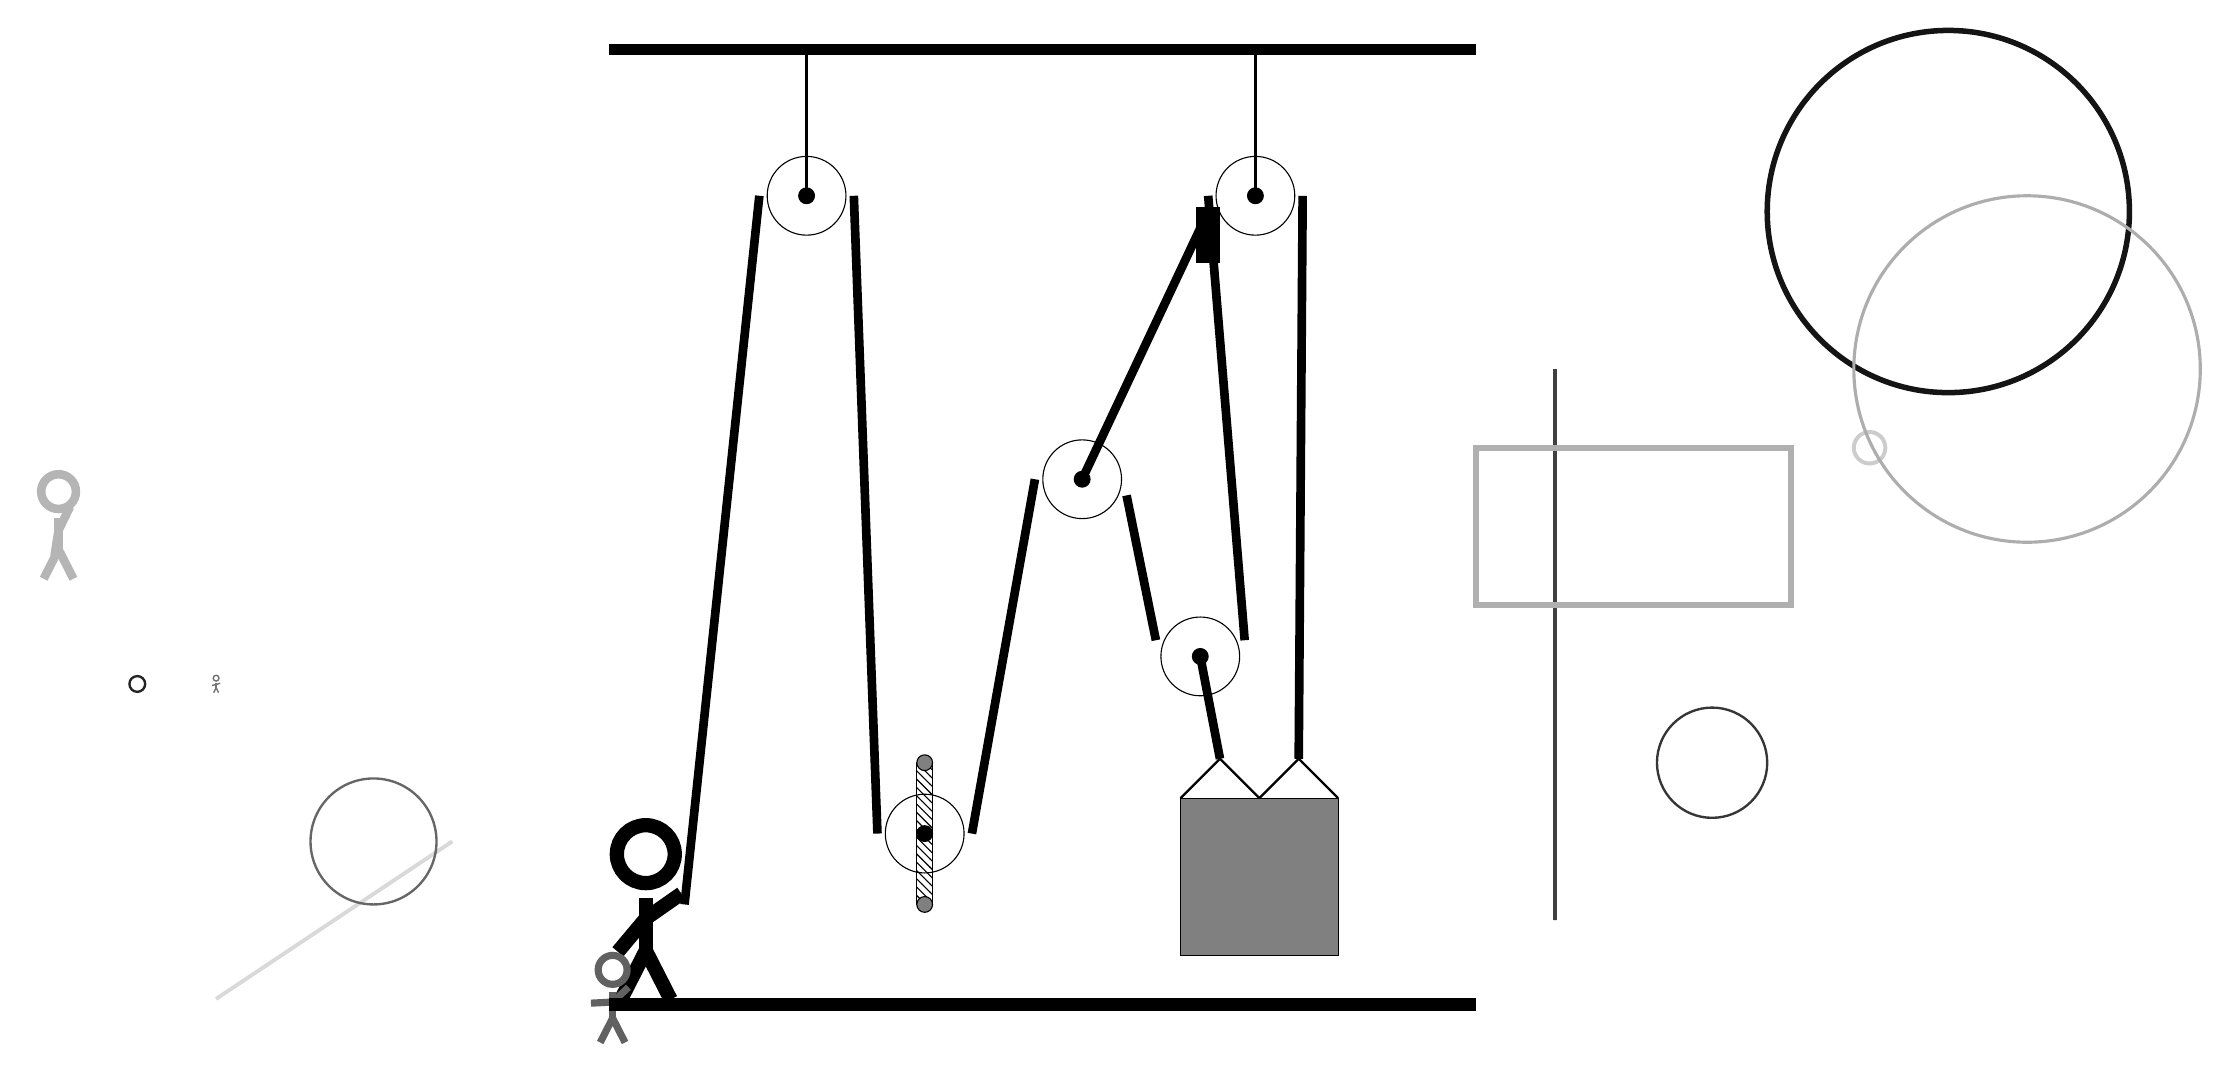
\begin{tikzpicture}
			%%%%% START %%%%%
			
			\draw[fill=black] (-6, 9) rectangle (5, 9.125);
			
			\draw (0, 3.6) circle (0.5);
			\draw[fill=black] (0, 3.6) circle (0.1);
			
			\draw (1.5, 1.35) circle (0.5);
			\draw[fill=black] (1.5, 1.35) circle (0.1);
			
			\draw (2.2, 7.2) circle (0.5);
			\draw[fill=black] (2.2, 7.2) circle (0.1);
			\draw[thick] (2.2, 7.2) -- (2.2, 9);
			
			\draw (-3.5, 7.2) circle (0.5);
			\draw[fill=black] (-3.5, 7.2) circle (0.1);
			\draw[thick] (-3.5, 7.2) -- (-3.5, 9);
			
			\draw (-2, -0.9) circle (0.5);
			\draw[fill=black] (-2, -0.9) circle (0.1);
			\draw[pattern=north west lines, pattern color=black] (-2.1, -0.0) rectangle (-1.9, -1.8);
			\draw[fill=black!50] (-2, -0.0) circle (0.1);
			\draw[fill=black!50] (-2, -1.8) circle (0.1);
			
			\draw[thick]  (1.25, -0.45) -- (1.75, 0.05) -- (2.25, -0.45) -- (2.75, 0.05) -- (3.25, -0.45);
			\draw[fill=black!50] (1.25, -0.45) rectangle (3.25, -2.45);
			\draw[line width=1.1mm] (-5.05, -1.8) -- (-4.1, 7.2);
			\centerarc[line width=1.1mm](-3.5, 7.2)(0:180:0.6);
			\draw[line width=1.1mm] (-2.9, 7.2) -- (-2.6, -0.9);
			\centerarc[line width=1.1mm](-2, -0.9)(180:360:0.6);
			\draw[line width=1.1mm] (-1.4, -0.9) -- (-0.6, 3.6);
			\draw[line width=1.1mm] (0, 3.6) -- (1.6, 7.0);
			\draw[line width=1.1mm, fill=black](1.5, 6.4) rectangle (1.7, 7.0);
			\centerarc[line width=1.1mm](0, 3.6)(-20:180:0.6);
			\draw[line width=1.1mm] (0.5638, 3.3948) -- (0.9362, 1.5552);
			
			\centerarc[line width=1.1mm](1.5, 1.35)(160:380:0.6);
			\draw[line width=1.1mm] (2.0638, 1.5552) -- (1.6, 7.2);
			\draw[line width=1.1mm](1.5, 1.35) -- (1.75, 0.05);
			\centerarc[line width=1.1mm](2.2, 7.2)(0:180:0.6);
			\draw[line width=1.1mm] (2.8, 7.2) -- (2.75, 0.05);
			
			\node at (-5.5, -1.9) {\Strichmaxerl[10][50][35]};
			
			\draw [line width=0.3mm, color=black!79](8, 0) circle (0.7);
			
			\draw[line width=0.5mm, color=black!15](-8, -1) -- (-11, -3);
			\draw [line width=0.3mm, color=black!86](-12, 1) circle (0.1);
			\draw [line width=0.3mm, color=black!60](-9, -1) circle (0.8);
			\draw[line width=0.5mm, color=black!75] (6, 5) rectangle (6, -2);
			
			\draw [line width=0.7mm, color=black!92](11, 7) circle (2.3);
			\node[line width=0.4mm, color=black!62] at (-6, -3) {\Strichmaxerl[5][3][43]};
			\draw[line width=0.7mm, color=black!31] (5, 4) rectangle (9, 2);
			\node[line width=0.6mm, color=black!29] at (-13, 3) {\Strichmaxerl[6][81][64]};
			
			\node[line width=0.2mm, color=black!54] at (-11, 1) {\Strichmaxerl[1][11][18]};
			
			\draw [line width=0.5mm, color=black!20](10, 4) circle (0.2);
			\draw [line width=0.4mm, color=black!32](12, 5) circle (2.2);
			
			\draw[fill=black] (-6, -3) rectangle (5, -3.15);
			
			%%%%% END %%%%%
		\end{tikzpicture}
	\end{figure}	
\end{document}